\documentclass[]{tufte-handout}

% ams
\usepackage{amssymb,amsmath}

\usepackage{ifxetex,ifluatex}
\usepackage{fixltx2e} % provides \textsubscript
\ifnum 0\ifxetex 1\fi\ifluatex 1\fi=0 % if pdftex
  \usepackage[T1]{fontenc}
  \usepackage[utf8]{inputenc}
\else % if luatex or xelatex
  \makeatletter
  \@ifpackageloaded{fontspec}{}{\usepackage{fontspec}}
  \makeatother
  \defaultfontfeatures{Ligatures=TeX,Scale=MatchLowercase}
  \makeatletter
  \@ifpackageloaded{soul}{
     \renewcommand\allcapsspacing[1]{{\addfontfeature{LetterSpace=15}#1}}
     \renewcommand\smallcapsspacing[1]{{\addfontfeature{LetterSpace=10}#1}}
   }{}
  \makeatother

\fi

% graphix
\usepackage{graphicx}
\setkeys{Gin}{width=\linewidth,totalheight=\textheight,keepaspectratio}

% booktabs
\usepackage{booktabs}

% url
\usepackage{url}

% hyperref
\usepackage{hyperref}

% units.
\usepackage{units}


\setcounter{secnumdepth}{-1}

% citations
\usepackage{natbib}
\bibliographystyle{plainnat}


% pandoc syntax highlighting
\usepackage{color}
\usepackage{fancyvrb}
\newcommand{\VerbBar}{|}
\newcommand{\VERB}{\Verb[commandchars=\\\{\}]}
\DefineVerbatimEnvironment{Highlighting}{Verbatim}{commandchars=\\\{\}}
% Add ',fontsize=\small' for more characters per line
\newenvironment{Shaded}{}{}
\newcommand{\AlertTok}[1]{\textcolor[rgb]{1.00,0.00,0.00}{\textbf{#1}}}
\newcommand{\AnnotationTok}[1]{\textcolor[rgb]{0.38,0.63,0.69}{\textbf{\textit{#1}}}}
\newcommand{\AttributeTok}[1]{\textcolor[rgb]{0.49,0.56,0.16}{#1}}
\newcommand{\BaseNTok}[1]{\textcolor[rgb]{0.25,0.63,0.44}{#1}}
\newcommand{\BuiltInTok}[1]{#1}
\newcommand{\CharTok}[1]{\textcolor[rgb]{0.25,0.44,0.63}{#1}}
\newcommand{\CommentTok}[1]{\textcolor[rgb]{0.38,0.63,0.69}{\textit{#1}}}
\newcommand{\CommentVarTok}[1]{\textcolor[rgb]{0.38,0.63,0.69}{\textbf{\textit{#1}}}}
\newcommand{\ConstantTok}[1]{\textcolor[rgb]{0.53,0.00,0.00}{#1}}
\newcommand{\ControlFlowTok}[1]{\textcolor[rgb]{0.00,0.44,0.13}{\textbf{#1}}}
\newcommand{\DataTypeTok}[1]{\textcolor[rgb]{0.56,0.13,0.00}{#1}}
\newcommand{\DecValTok}[1]{\textcolor[rgb]{0.25,0.63,0.44}{#1}}
\newcommand{\DocumentationTok}[1]{\textcolor[rgb]{0.73,0.13,0.13}{\textit{#1}}}
\newcommand{\ErrorTok}[1]{\textcolor[rgb]{1.00,0.00,0.00}{\textbf{#1}}}
\newcommand{\ExtensionTok}[1]{#1}
\newcommand{\FloatTok}[1]{\textcolor[rgb]{0.25,0.63,0.44}{#1}}
\newcommand{\FunctionTok}[1]{\textcolor[rgb]{0.02,0.16,0.49}{#1}}
\newcommand{\ImportTok}[1]{#1}
\newcommand{\InformationTok}[1]{\textcolor[rgb]{0.38,0.63,0.69}{\textbf{\textit{#1}}}}
\newcommand{\KeywordTok}[1]{\textcolor[rgb]{0.00,0.44,0.13}{\textbf{#1}}}
\newcommand{\NormalTok}[1]{#1}
\newcommand{\OperatorTok}[1]{\textcolor[rgb]{0.40,0.40,0.40}{#1}}
\newcommand{\OtherTok}[1]{\textcolor[rgb]{0.00,0.44,0.13}{#1}}
\newcommand{\PreprocessorTok}[1]{\textcolor[rgb]{0.74,0.48,0.00}{#1}}
\newcommand{\RegionMarkerTok}[1]{#1}
\newcommand{\SpecialCharTok}[1]{\textcolor[rgb]{0.25,0.44,0.63}{#1}}
\newcommand{\SpecialStringTok}[1]{\textcolor[rgb]{0.73,0.40,0.53}{#1}}
\newcommand{\StringTok}[1]{\textcolor[rgb]{0.25,0.44,0.63}{#1}}
\newcommand{\VariableTok}[1]{\textcolor[rgb]{0.10,0.09,0.49}{#1}}
\newcommand{\VerbatimStringTok}[1]{\textcolor[rgb]{0.25,0.44,0.63}{#1}}
\newcommand{\WarningTok}[1]{\textcolor[rgb]{0.38,0.63,0.69}{\textbf{\textit{#1}}}}

% longtable
\usepackage{longtable,booktabs}

% multiplecol
\usepackage{multicol}

% strikeout
\usepackage[normalem]{ulem}

% morefloats
\usepackage{morefloats}


% tightlist macro required by pandoc >= 1.14
\providecommand{\tightlist}{%
  \setlength{\itemsep}{0pt}\setlength{\parskip}{0pt}}

% title / author / date
\title[分散の加法性を視覚的に理解する]{分散の加法性を視覚的に理解する}
\author{Sampo Suzuki, CC 4.0 BY-NC-SA}
\date{2021-05-31}

% --- 参考資料 ----------------------------------------------------------------
% https://github.com/Gedevan-Aleksizde/Japan.R2019/blob/master/latex/preamble.tex
% https://teastat.blogspot.com/2019/01/bookdown.html

% --- Packages ----------------------------------------------------------------
% 日本語とtufte, kableExtraを使うために必要なTeXパッケージ指定
% tufteではA4サイズの指定が不可能
%  A4 210mm x 297mm
%   \usepackage[a4paper, total={6.5in, 9.5in}]{geometry}
%   \usepackage{indentfirst}   # tinytexのリポジトリには存在しない?
% \usepackage[a4paper, total={160mm, 247mm}, left=25mm, top=25mm]{geometry}
% \usepackage[pdfbox,tombo]{gentombow}  % トンボを設定する場合は有効にする
% \usepackage{ifthen}                     % 条件分岐用 \ifthenelse{条件}{T}{F}
\usepackage{booktabs}                   % ここからkableExtra用パッケージ
\usepackage{longtable}                  % 
\usepackage{array}                      % 
\usepackage{multirow}                   % 
\usepackage{wrapfig}                    % 
\usepackage{float}                      % 
\usepackage{colortbl}                   % 
\usepackage{pdflscape}                  % 
\usepackage{tabu}                       % 
\usepackage{threeparttable}             % 
\usepackage{threeparttablex}            % 
\usepackage[normalem]{ulem}             % 
\usepackage{inputenc}                   % 
\usepackage{makecell}                   % 
\usepackage{xcolor}                     % ここまでkableExtra用
\usepackage{amsmath}                    % 
\usepackage{fontawesome5}               % fontawesomeを使うために必要
\usepackage{subfig}
\usepackage{xeCJK}                      % 以下、日本語フォント用に必要
% \usepackage[noto]{zxjafont}             % Linux環境ではこちを指定
\usepackage[haranoaji]{zxjafont}      % Windows環境ではこちらを指定する
\usepackage{zxjatype}
\usepackage{pxrubrica}                  % ルビ用
\usepackage{hyperref}                   % ハイパーリンク用必要?

% --- Index ------------------------------------------------------------------
% https://texwiki.texjp.org/?%E7%B4%A2%E5%BC%95%E4%BD%9C%E6%88%90
% これを指定するとIndex(索引)は作成されるが参照ページがズレる
% 中間ファイルの.indではページはズレていないので、その後の結合処理がおかしい
% \usepackage{makeidx}
% \makeindex
% \usepackage{showidx}                  % 索引確認用

% --- Table of Contentes ------------------------------------------------------
% TOCにLOT(List of Tables), LOF(List of Figures), Bibliography, Indexを表示
% \usepackage[nottoc]{tocbibind}

% --- Fonts -------------------------------------------------------------------
% フォントしては index.html でも可能(pandoc用オプションは index.htmlにて)
% \setCJKmonofont{Source Han Code JP}
% \setmonofont{Source Han Code JP}     % Linuxではこれのみコメントアウトする
% \setjamonofont{Source Han Code JP}

% ## 日本語フォントの扱いについてはzxjafontパッケージの解説を参照のこと
% # https://mirror.las.iastate.edu/tex-archive/language/japanese/zxjafont/zxjafont.pdf
% #
% ## Windows環境ではなぜかNotoフォントが認識されないので源ノシリーズベースの
% ## 原ノ味フォントかIPAexフォントを利用する(原ノ味はtlmgrでインストール可)
% # \usepackage[haranoaji]{zxjafont}
% # \usepackage[ipaex]{zxjafont}
% #
% ## Windows環境でNotoフォントを指定したい場合は以下のようにheader-includeで
% ## 個別に指定する(setCJKxxxfotnの指定は必要?)
% # \setmainfont{NotoSerifCJKjp-Regular.otf}[BoldFont=NotoSerifCJKjp-Bold.otf]
% # \setsansfont{NotoSansCJKjp-Regular.otf}[BoldFont=NotoSansCJKjp-Bold.otf]
% # \setmonofont{NotoSansMonoCJKjp-Regular.otf}[BoldFont=NotoSansMonoCJKjp-Bold.otf]
% ## モノフォントは源ノ角コード(Source Code Proの日本語版)がおすゝめ
% # \setmonofont{SourceHanCodeJP-Regular.otf}[BoldFont=SourceHanCodeJPS-Bold.otf]

\begin{document}

\maketitle




\hypertarget{introduction}{%
\section{\texorpdfstring{\textbf{Introduction}}{Introduction}}\label{introduction}}

 2021年度データ分析勉強会のテキストである『統計解析のはなし』\citep{ToukeiKaisekinoHanashi}の「標本が2つになれば」(P26〜)には分散の加法性の話が出てきます。分散の加法性は理解できるようでいて、理解できていないので、\textbf{R}を使って分散の加法性を可視化しながら説明してみます。

以降、平均値\(\mu\)、標準偏差\(\sigma\)、分散\(\sigma^2\)である正規分布を\(N(\mu, \sigma^2)\)と表記します。

 

\hypertarget{ux52a0ux6cd5ux6027ux3092ux53efux8996ux5316ux3059ux308b}{%
\section{\texorpdfstring{\textbf{加法性を可視化する}}{加法性を可視化する}}\label{ux52a0ux6cd5ux6027ux3092ux53efux8996ux5316ux3059ux308b}}

 以下の平均値と標準偏差を持つ二つの正規分布を\texttt{rnorm()}関数による正規分布乱数を用いて作成\footnote{n
  = \ensuremath{5\times 10^{6}}個の値を作成しています}します。

\begin{longtable}[]{@{}lccl@{}}
\caption{二つの正規分布}\tabularnewline
\toprule
正規分布 & 平均 & 標準偏差 & 備考 \\
\midrule
\endfirsthead
\toprule
正規分布 & 平均 & 標準偏差 & 備考 \\
\midrule
\endhead
\(N(\mu_a, \sigma^2_a)\) & \(\mu_a = 10\) & \(\sigma_a = 10\) & \\
\(N(\mu_b, \sigma^2_b)\) & \(\mu_b = 30\) & \(\sigma_b = 10\) & \\
\bottomrule
\end{longtable}

\begin{Shaded}
\begin{Highlighting}[numbers=left,,]
\NormalTok{a }\OtherTok{\textless{}{-}} \FunctionTok{rnorm}\NormalTok{(n, }\AttributeTok{mean =} \DecValTok{10}\NormalTok{, }\AttributeTok{sd =} \DecValTok{10}\NormalTok{)}
\NormalTok{b }\OtherTok{\textless{}{-}} \FunctionTok{rnorm}\NormalTok{(n, }\AttributeTok{mean =} \DecValTok{30}\NormalTok{, }\AttributeTok{sd =} \DecValTok{10}\NormalTok{)}
\end{Highlighting}
\end{Shaded}

\begin{marginfigure}

{\centering 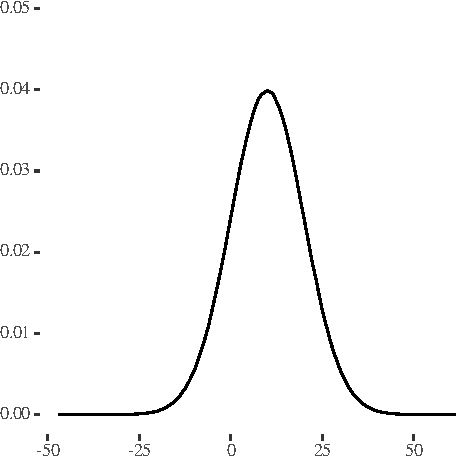
\includegraphics{AdditivityOfVariance_files/figure-latex/unnamed-chunk-2-1} 

}

\caption[$N(\mu_a, \sigma^2_a)$の分布]{$N(\mu_a, \sigma^2_a)$の分布}\label{fig:unnamed-chunk-2}
\end{marginfigure}

\begin{marginfigure}

{\centering 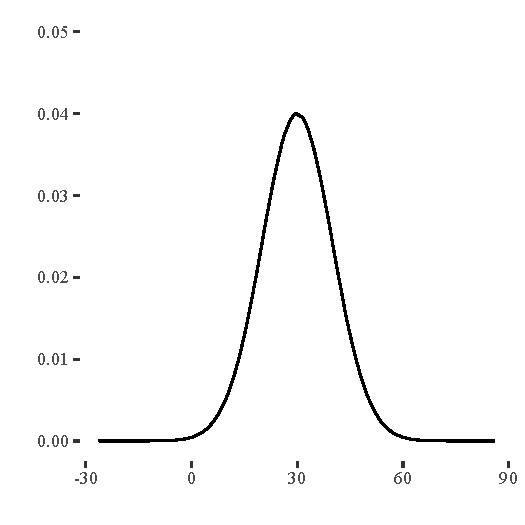
\includegraphics{AdditivityOfVariance_files/figure-latex/unnamed-chunk-3-1} 

}

\caption[$N(\mu_b, \sigma^2_bb)$の分布]{$N(\mu_b, \sigma^2_bb)$の分布}\label{fig:unnamed-chunk-3}
\end{marginfigure}

\begin{longtable}[]{@{}lcccl@{}}
\caption{二つの正規分布の要約統計量}\tabularnewline
\toprule
正規分布 & 平均 & 分散 & 標準偏差 & 備考 \\
\midrule
\endfirsthead
\toprule
正規分布 & 平均 & 分散 & 標準偏差 & 備考 \\
\midrule
\endhead
\(N(\mu_a, \sigma^2_a)\) & 10.0014697 & 100.0509323 & 10.0025463 & \\
\(N(\mu_b, \sigma^2_b)\) & 30.0075917 & 100.083893 & 10.0041938 & \\
\bottomrule
\end{longtable}

この二つの正規分布\(N(\mu_a, \sigma^2_a)\)と\(N(\mu_b,\sigma^2_b)\)からランダムサンプリングにより一つずづ値を取り出して加算します。すなわち
 
\[N(\mu_a, \sigma^2_a)\mbox{ から取り出した値} + N(\mu_b,\sigma^2_b)\mbox{ から取り出した値}\]

という新しい値を作成します。取り出した値は元に戻し、同様の取り出し、加算を繰り返すと以下のようなデータが作成できます。ここではスペースの都合で先頭から限定して表示しています。

\begin{Shaded}
\begin{Highlighting}[numbers=left,,]
\NormalTok{c }\OtherTok{\textless{}{-}} \FunctionTok{c}\NormalTok{(}\FunctionTok{sample}\NormalTok{(a, n, }\AttributeTok{replace =} \ConstantTok{TRUE}\NormalTok{) }\SpecialCharTok{+} \FunctionTok{sample}\NormalTok{(b, n, }\AttributeTok{replace =} \ConstantTok{TRUE}\NormalTok{))}
\FunctionTok{head}\NormalTok{(c, }\DecValTok{50}\NormalTok{)}
\end{Highlighting}
\end{Shaded}

\begin{verbatim}
##  [1] 30.266543 33.482135 33.883714 52.912233 47.582459 25.639092 39.881634
##  [8] 14.988764 51.345507 36.475710 44.235409 45.972599 37.013345 32.812017
## [15] 14.516596 64.263308 44.186538 43.642677 21.244094 19.564546 47.347405
## [22] 58.728940 21.215430 32.750743 38.887516 29.302033 49.807043 26.356846
## [29] 23.281160 36.135680 44.107899 47.692939 16.805313 54.466007 37.318704
## [36] 23.799790 62.604869 30.765222  4.836705 53.636457 46.941686 48.839953
## [43] 46.173439 43.040911  9.799147 35.184573 19.722850 45.581071 53.556008
## [50] 49.641749
\end{verbatim}

分散の加法性により上記のデータは\(N(\mu_a + \mu_b, \sigma^2_a + \sigma^2_b))\)という正規分布になるはずですが実際はどうでしょう。各正規分布の平均値と分散を比較します。

\begin{longtable}[]{@{}lccl@{}}
\caption{各分布の要約統計量}\tabularnewline
\toprule
正規分布 & 平均 & 分散 & 備考 \\
\midrule
\endfirsthead
\toprule
正規分布 & 平均 & 分散 & 備考 \\
\midrule
\endhead
\(N(\mu_a, \sigma^2_a)\) & 10.0014697 & 100.0509323 & 元の分布 \\
\(N(\mu_b, \sigma^2_b)\) & 30.0075917 & 100.083893 & 元の分布 \\
\(N(\mu_a + \mu_b, \sigma^2_a + \sigma^2_b))\) & 40.0090615 &
200.1348252 & 分散の加法性 \\
\(N(\mu_c, \sigma^2_c)\) & 40.0054096 & 200.1730197 & 実際の分布 \\
\bottomrule
\end{longtable}

このように確かに分散の加法性が成り立っており、正規分布\(N(\mu_a, \sigma^2_a)\)や\(N(\mu_b,\sigma^2_b)\)より横に広がった正規分布になっていることが分かります。

\begin{marginfigure}

{\centering 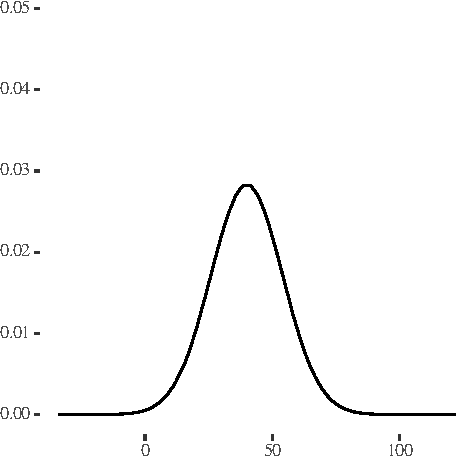
\includegraphics{AdditivityOfVariance_files/figure-latex/unnamed-chunk-5-1} 

}

\caption[$N(\mu_c, \sigma^2_c)$の分布]{$N(\mu_c, \sigma^2_c)$の分布}\label{fig:unnamed-chunk-5}
\end{marginfigure}

\newpage

\hypertarget{ux540cux4e00ux306eux6b63ux898fux5206ux5e03ux304bux3089ux53d6ux308aux51faux3057ux5024ux3092ux52a0ux7b97ux3057ux305fux5834ux5408}{%
\subsection{\texorpdfstring{\textbf{同一の正規分布から取り出し値を加算した場合}}{同一の正規分布から取り出し値を加算した場合}}\label{ux540cux4e00ux306eux6b63ux898fux5206ux5e03ux304bux3089ux53d6ux308aux51faux3057ux5024ux3092ux52a0ux7b97ux3057ux305fux5834ux5408}}

 次に二つの正規分布\(N(\mu_a, \sigma^2_a)\)と\(N(\mu_b,\sigma^2_b)\)がまったく等しいと仮定します。つまり

\[\mu_a = \mu_b = \mu_d\]

\[\sigma_a = \sigma_b = \sigma_d\]

という正規分布\(N(\mu_d, \sigma^2_d)\)を作成します。

\begin{Shaded}
\begin{Highlighting}[numbers=left,,]
\NormalTok{d }\OtherTok{\textless{}{-}} \FunctionTok{rnorm}\NormalTok{(n, }\AttributeTok{mean =} \DecValTok{10}\NormalTok{, }\AttributeTok{sd =} \DecValTok{10}\NormalTok{)}
\FunctionTok{head}\NormalTok{(d, }\DecValTok{50}\NormalTok{)}
\end{Highlighting}
\end{Shaded}

\begin{verbatim}
##  [1]  16.8747940  -3.5899771  15.4848762  -5.8108516  21.3126299  -2.6923281
##  [7]  19.8018776  17.5592976  18.1182472  12.4138245  26.0172186  15.7833011
## [13]  -0.2765988  15.3199164  17.7032323  13.0090420  11.2049580  10.3761903
## [19]   5.6129375   6.4848689   4.5988170   0.4041192 -11.9968756   8.3380746
## [25]   5.0284415   4.0519065  18.8237080  -5.4725188   6.9070690  18.8567418
## [31]   1.0479369   0.8552902  26.4492488  21.7604984  12.3795891   9.8857552
## [37]  11.1948368   5.2856539   0.8707844   4.9711472  32.6614360  11.3779946
## [43]  27.2907066  28.1782244   9.1747638  -3.0257148   4.8021001  -2.8516725
## [49]  19.9887135  28.0180779
\end{verbatim}

この正規分布\(N(\mu_d, \sigma^2_d)\)から先程と同様にランダムサンプリングにより一つずづ値を取り出して加算しますが、今回は同一正規分布\(N(\mu_d, \sigma^2_d)\)ですので、二つ取り出します。取り出した値は元の正規分布に戻し同様の操作を繰り返します。

 

\begin{Shaded}
\begin{Highlighting}[numbers=left,,]
\NormalTok{e }\OtherTok{\textless{}{-}} \FunctionTok{c}\NormalTok{(}\FunctionTok{sample}\NormalTok{(d, n, }\AttributeTok{replace =} \ConstantTok{TRUE}\NormalTok{) }\SpecialCharTok{+} \FunctionTok{sample}\NormalTok{(d, n, }\AttributeTok{replace =} \ConstantTok{TRUE}\NormalTok{))}
\FunctionTok{head}\NormalTok{(e, }\DecValTok{50}\NormalTok{)}
\end{Highlighting}
\end{Shaded}

\begin{verbatim}
##  [1]  35.6145534  15.0076269  21.8897246  13.8629208  20.3446667  27.3814441
##  [7]   2.8956442  18.0596505  23.8732482  -4.9288152  -2.2386834  28.9913052
## [13]  35.0330880  -8.5718351   5.7975086  35.9766988   3.6891855  12.7828574
## [19]  -1.8057183  24.7751618  36.0577628  14.5431025  40.8758199  15.9372723
## [25]  23.4557804  23.6267963  17.2804571  -3.1691862   9.3926850  16.7604507
## [31]  34.4599675   9.8516480   2.7117987  23.1990931  -4.7609045  23.1869043
## [37]  31.0536844  34.1684054 -11.7905499  25.4874906  18.1658356   2.9928224
## [43]  25.4289769  13.9323886  22.9294320  14.7481540  54.4881718  15.7111684
## [49]  34.4770169  -0.3311999
\end{verbatim}

\newpage

分散の加法性により以下が成り立ちます。

\[N(\mu_d + \mu_d, \sigma^2_d + \sigma^2_d) = N(2\mu_d, 2\sigma^2_d)\]

つまり、正規分布\(N(\mu_d, \sigma^2_d)\)から取り出した二つの値の和である正規分布\(N(\mu_e, \sigma^2_e)\)は

\begin{longtable}[]{@{}
  >{\raggedright\arraybackslash}p{(\columnwidth - 8\tabcolsep) * \real{0.16}}
  >{\centering\arraybackslash}p{(\columnwidth - 8\tabcolsep) * \real{0.20}}
  >{\centering\arraybackslash}p{(\columnwidth - 8\tabcolsep) * \real{0.20}}
  >{\centering\arraybackslash}p{(\columnwidth - 8\tabcolsep) * \real{0.36}}
  >{\raggedright\arraybackslash}p{(\columnwidth - 8\tabcolsep) * \real{0.09}}@{}}
\caption{加法性による要約統計量}\tabularnewline
\toprule
正規分布 & 平均 & 分散 & 標準偏差 & 備考 \\
\midrule
\endfirsthead
\toprule
正規分布 & 平均 & 分散 & 標準偏差 & 備考 \\
\midrule
\endhead
\(N(\mu_e, \sigma^2_e)\) & \(2 \mu_d\) & \(2 \sigma^2_d\) &
\(\sqrt{2 \sigma^2_d} = \sqrt{2}\sigma_d\) & \\
\bottomrule
\end{longtable}

という正規分布をすることになります。加法性と実際の正規分布を比べてみると

\begin{longtable}[]{@{}lccl@{}}
\caption{各分布の要約統計量}\tabularnewline
\toprule
正規分布 & 平均 & 分散 & 備考 \\
\midrule
\endfirsthead
\toprule
正規分布 & 平均 & 分散 & 備考 \\
\midrule
\endhead
\(N(\mu_d, \sigma^2_d)\) & 10.010013 & 99.9432245 & 元の分布 \\
\(N(2\mu_d, 2\sigma^2_d)\) & 20.020026 & 199.8864489 & 分散の加法性 \\
\(N(\mu_e, \sigma^2_e)\) & 20.0121122 & 199.861238 & 実際の分布 \\
\bottomrule
\end{longtable}

となり、同一正規分布の場合でも分散の加法性が成り立っていることが分かります。

\begin{marginfigure}

{\centering 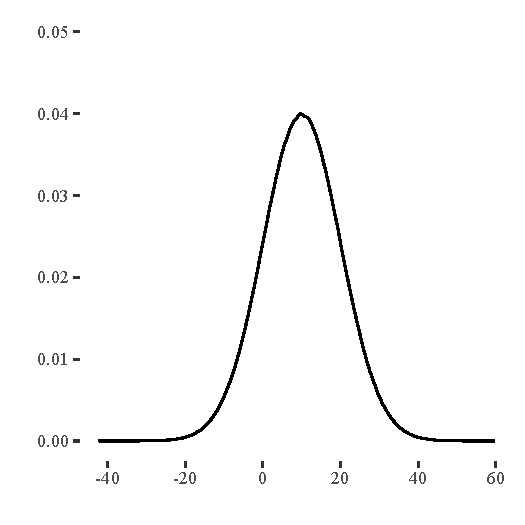
\includegraphics{AdditivityOfVariance_files/figure-latex/unnamed-chunk-8-1} 

}

\caption[$N(\mu_d, \sigma^2_d)$の分布]{$N(\mu_d, \sigma^2_d)$の分布}\label{fig:unnamed-chunk-8}
\end{marginfigure}

\begin{marginfigure}

{\centering 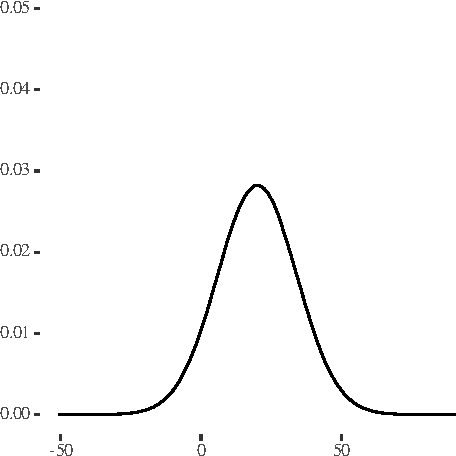
\includegraphics{AdditivityOfVariance_files/figure-latex/unnamed-chunk-9-1} 

}

\caption[$N(\mu_e, \sigma^2_e)$の分布]{$N(\mu_e, \sigma^2_e)$の分布}\label{fig:unnamed-chunk-9}
\end{marginfigure}

\newpage

\hypertarget{ux540cux4e00ux306eux6b63ux898fux5206ux5e03ux304bux3089ux53d6ux308aux51faux3057ux305fux5024ux3092ux5e73ux5747ux3057ux305fux5834ux5408}{%
\subsection{\texorpdfstring{\textbf{同一の正規分布から取り出した値を平均した場合}}{同一の正規分布から取り出した値を平均した場合}}\label{ux540cux4e00ux306eux6b63ux898fux5206ux5e03ux304bux3089ux53d6ux308aux51faux3057ux305fux5024ux3092ux5e73ux5747ux3057ux305fux5834ux5408}}

 同一の正規分布\(N(\mu_d, \sigma^2_d)\)から取り出した二つの値の\textbf{平均値の分布}を考えてみます。「二つの値の平均値の平均値」とは、正規分布\(N(\mu_d, \sigma^2_d)\)から、ランダムサンプリングで二つの値を取り出して、その平均値を取るということです。取り出した値は元の正規分布へ戻し、同様の操作を繰り返します。

\begin{Shaded}
\begin{Highlighting}[numbers=left,,]
\NormalTok{f }\OtherTok{\textless{}{-}} \FunctionTok{c}\NormalTok{((}\FunctionTok{sample}\NormalTok{(d, n, }\AttributeTok{replace =} \ConstantTok{TRUE}\NormalTok{) }\SpecialCharTok{+} \FunctionTok{sample}\NormalTok{(d, n, }\AttributeTok{replace =} \ConstantTok{TRUE}\NormalTok{)) }\SpecialCharTok{/} \DecValTok{2}\NormalTok{)}
\FunctionTok{head}\NormalTok{(f, }\DecValTok{20}\NormalTok{)}
\end{Highlighting}
\end{Shaded}

\begin{verbatim}
##  [1] 14.5186470  8.2265162  0.9118885 11.8694537  7.7600256  5.0938372
##  [7]  3.8634928 20.9747932  0.4723029  4.0771369 12.8340336  9.6796570
## [13] 11.4256020 18.7724639 14.6823738  5.8606737  3.7060742  7.1215704
## [19]  7.8065397  6.9345260
\end{verbatim}

この正規分布正規分布\(N(\mu_f, \sigma^2_f)\)は、二つの値の平均値、つまり二つの値を半分に割った値ですので正規分布\(N(2\mu_d, 2\sigma^2_d)\)のすべての値を半分にした正規分布になると予想できます。

\[\mbox{「二つの標本の平均値」の平均値} = \frac{2\mu_d}{2} = \mu_d\]

\[\mbox{「二つの標本の平均値」の標準偏差} = \frac{\sqrt{2}\sigma_d}{2} = \frac{\sigma_d}{\sqrt{2}}\]

\[\mbox{「二つの標本の平均値」の分散} = (\frac{\sigma_d}{\sqrt{2}})^2 = \frac{\sigma^2_d}{2}\]

\begin{marginfigure}

{\centering 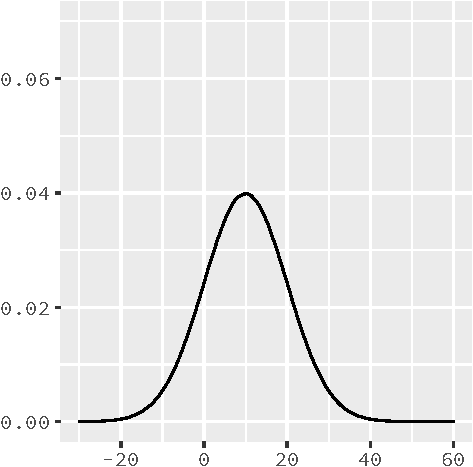
\includegraphics{AdditivityOfVariance_files/figure-latex/unnamed-chunk-11-1} 

}

\caption[$N(\mu_d, \sigma^2_d)$の分布]{$N(\mu_d, \sigma^2_d)$の分布}\label{fig:unnamed-chunk-11}
\end{marginfigure}

\begin{marginfigure}

{\centering 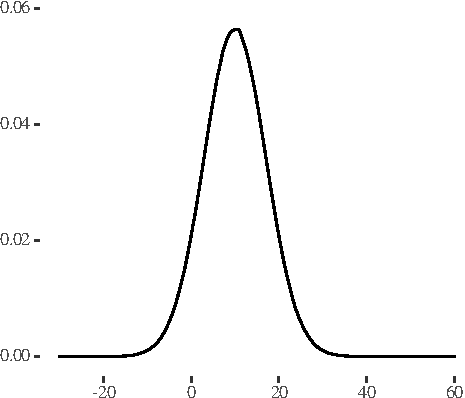
\includegraphics{AdditivityOfVariance_files/figure-latex/unnamed-chunk-12-1} 

}

\caption[$N(\mu_f, \sigma^2_f)$の分布]{$N(\mu_f, \sigma^2_f)$の分布}\label{fig:unnamed-chunk-12}
\end{marginfigure}

\begin{longtable}[]{@{}lcccl@{}}
\caption{各分布の要約統計量}\tabularnewline
\toprule
正規分布 & 平均 & 分散 & 標準偏差 & 備考 \\
\midrule
\endfirsthead
\toprule
正規分布 & 平均 & 分散 & 標準偏差 & 備考 \\
\midrule
\endhead
\(N(\mu_d, \sigma^2_d)\) & 10.010013 & 99.9432245 & 9.9971608 &
元の分布 \\
\(N(\mu_d, \frac{\sigma^2_d}{2})\) & 10.010013 & 49.9716122 & 7.0690602
& 分散の加法性 \\
\(N(\mu_f, \sigma^2_f)\) & 10.0107453 & 49.9630623 & 7.0684554 &
実際の分布 \\
\bottomrule
\end{longtable}

このように元の分布よりも鋭い分布になっていることがわかります。

\newpage

\hypertarget{ux4e09ux3064ux5024ux306eux5e73ux5747ux5024ux306eux5834ux5408}{%
\subsection{\texorpdfstring{\textbf{三つ値の平均値の場合}}{三つ値の平均値の場合}}\label{ux4e09ux3064ux5024ux306eux5e73ux5747ux5024ux306eux5834ux5408}}

 次に同一の正規分布\(N(\mu_d, \sigma^2_d)\)から取り出した三つの値の\textbf{平均値の分布}を考えてみます。
 

\begin{Shaded}
\begin{Highlighting}[numbers=left,,]
\NormalTok{g }\OtherTok{\textless{}{-}} \FunctionTok{c}\NormalTok{((}\FunctionTok{sample}\NormalTok{(d, n, }\AttributeTok{replace =} \ConstantTok{TRUE}\NormalTok{) }\SpecialCharTok{+} \FunctionTok{sample}\NormalTok{(d, n, }\AttributeTok{replace =} \ConstantTok{TRUE}\NormalTok{) }
        \SpecialCharTok{+} \FunctionTok{sample}\NormalTok{(d, n, }\AttributeTok{replace =} \ConstantTok{TRUE}\NormalTok{)) }\SpecialCharTok{/} \DecValTok{3}\NormalTok{)}
\FunctionTok{head}\NormalTok{(g, }\DecValTok{20}\NormalTok{)}
\end{Highlighting}
\end{Shaded}

\begin{verbatim}
##  [1]  7.139431  9.887220 -4.155243 18.828068 15.765168  8.794437  9.583071
##  [8] 14.249243 22.482970 16.575414  6.892754  3.594099  4.213178  3.021689
## [15] 11.354231 16.786813 10.121512  3.710317  9.412671 10.026391
\end{verbatim}

\begin{longtable}[]{@{}lcccl@{}}
\caption{各分布の要約統計量}\tabularnewline
\toprule
正規分布 & 平均 & 分散 & 標準偏差 & 備考 \\
\midrule
\endfirsthead
\toprule
正規分布 & 平均 & 分散 & 標準偏差 & 備考 \\
\midrule
\endhead
\(N(\mu_d, \sigma^2_d)\) & 10.010013 & 99.9432245 & 9.9971608 &
元の分布 \\
\(N(\mu_g, \sigma^2_g)\) & 10.0080413 & 33.3303573 & 5.773245 &
実際の分布 \\
比率 & 0.999803 & 0.3334929 & 0.5774885 & 元の分布に対する比率 \\
\bottomrule
\end{longtable}

標準偏差の比率(0.5774885)は、\(\frac{1}{\sqrt{3}} = 0.5773503\)とほぼ等しいことが分かります。これより

\[N(\mu_g, \sigma^2_g) = N(\mu_d, \frac{\sigma^2_d}{3})\]

となることがわかります。

\begin{marginfigure}

{\centering 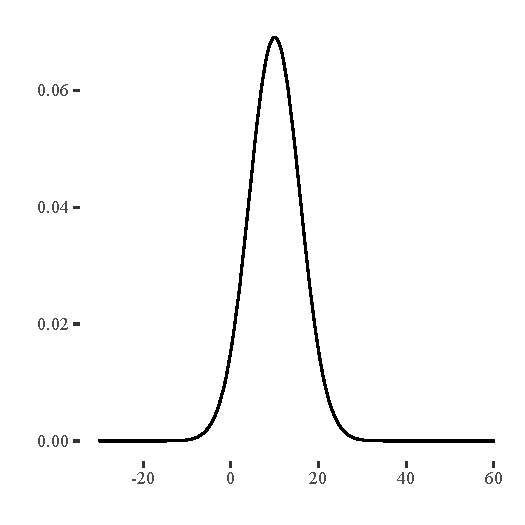
\includegraphics{AdditivityOfVariance_files/figure-latex/unnamed-chunk-14-1} 

}

\caption[$N(\mu_g, \sigma^2_g)$の分布]{$N(\mu_g, \sigma^2_g)$の分布}\label{fig:unnamed-chunk-14}
\end{marginfigure}

 

\hypertarget{ux4e00ux822cux5316ux3059ux308bux3068}{%
\subsection{\texorpdfstring{\textbf{一般化すると}}{一般化すると}}\label{ux4e00ux822cux5316ux3059ux308bux3068}}

 同一正規分布\(N(\mu, \sigma^2)\)から取り出した\(n\)個の値の\textbf{平均値の分布}\(N(\mu_, \sigma^2_n)\)は

\[N(\mu_n, \sigma^2_n) = N(\mu, \frac{\sigma^2}{n})\]

であり、平均は変わらず標準偏差が\(\frac{\sigma}{\sqrt{n}}\)となります。

\newpage

\hypertarget{ux304aux307eux3051ux5c0fux5ba4ux5148ux751fux306eux30a2ux30c9ux30d0ux30a4ux30b9ux304bux3089}{%
\section{\texorpdfstring{\textbf{おまけ}(小室先生のアドバイスから)}{おまけ(小室先生のアドバイスから)}}\label{ux304aux307eux3051ux5c0fux5ba4ux5148ux751fux306eux30a2ux30c9ux30d0ux30a4ux30b9ux304bux3089}}

 分散の加法性が成り立つには「データが独立」であるという前提条件があります。データが独立ということはデータ間の相関はないはずなので、乱数生成した二つのデータが本当に独立(無相関)なのかを確認します。

\begin{Shaded}
\begin{Highlighting}[numbers=left,,]
\NormalTok{f }\OtherTok{\textless{}{-}} \ControlFlowTok{function}\NormalTok{(}\AttributeTok{n =} \DecValTok{5000000}\NormalTok{) \{}
  \CommentTok{\# 乱数生成したデータ}
\NormalTok{  x }\OtherTok{\textless{}{-}} \FunctionTok{rnorm}\NormalTok{(}\AttributeTok{n =}\NormalTok{ n, }\AttributeTok{mean =} \DecValTok{10}\NormalTok{, }\AttributeTok{sd =} \DecValTok{10}\NormalTok{)}
\NormalTok{  y }\OtherTok{\textless{}{-}} \FunctionTok{rnorm}\NormalTok{(}\AttributeTok{n =}\NormalTok{ n, }\AttributeTok{mean =} \DecValTok{30}\NormalTok{, }\AttributeTok{sd =} \DecValTok{10}\NormalTok{)}
  \CommentTok{\# 乱数生成したデータ間の無相関の検定結果をデータフレーム化}
  \FunctionTok{cor.test}\NormalTok{(x, y) }\SpecialCharTok{\%\textgreater{}\%}\NormalTok{ broom}\SpecialCharTok{::}\FunctionTok{tidy}\NormalTok{()}
\NormalTok{\}}
\end{Highlighting}
\end{Shaded}

上記の関数を繰り返し実行し結果を表示します。

\begin{Shaded}
\begin{Highlighting}[numbers=left,,]
\NormalTok{df }\OtherTok{\textless{}{-}} \FunctionTok{data.frame}\NormalTok{()}
\ControlFlowTok{for}\NormalTok{ (i }\ControlFlowTok{in} \FunctionTok{c}\NormalTok{(}\DecValTok{1}\SpecialCharTok{:}\DecValTok{100}\NormalTok{)) \{}
\NormalTok{  df }\OtherTok{\textless{}{-}}\NormalTok{ dplyr}\SpecialCharTok{::}\FunctionTok{bind\_rows}\NormalTok{(df, }\FunctionTok{f}\NormalTok{())}
\NormalTok{\}}

\NormalTok{df }\SpecialCharTok{\%\textgreater{}\%} 
\NormalTok{  dplyr}\SpecialCharTok{::}\FunctionTok{select}\NormalTok{(conf.low, }\AttributeTok{corr =}\NormalTok{ estimate, conf.high,}
\NormalTok{                p.value, }\AttributeTok{t.value =}\NormalTok{ statistic) }\SpecialCharTok{\%\textgreater{}\%} 
\NormalTok{  knitr}\SpecialCharTok{::}\FunctionTok{kable}\NormalTok{()}
\end{Highlighting}
\end{Shaded}

\begin{longtable}[]{@{}rrrrr@{}}
\toprule
conf.low & corr & conf.high & p.value & t.value \\
\midrule
\endhead
-0.0004348 & 0.0004417 & 0.0013182 & 0.3232938 & 0.9877120 \\
-0.0006838 & 0.0001927 & 0.0010693 & 0.6664924 & 0.4309670 \\
-0.0018274 & -0.0009509 & -0.0000743 & 0.0334889 & -2.1261733 \\
-0.0006977 & 0.0001788 & 0.0010553 & 0.6893357 & 0.3997567 \\
-0.0013735 & -0.0004970 & 0.0003795 & 0.2664215 & -1.1113414 \\
-0.0005264 & 0.0003501 & 0.0012266 & 0.4337445 & 0.7828002 \\
-0.0007326 & 0.0001439 & 0.0010205 & 0.7475772 & 0.3218357 \\
-0.0010779 & -0.0002014 & 0.0006751 & 0.6524230 & -0.4503987 \\
-0.0007045 & 0.0001720 & 0.0010485 & 0.7005527 & 0.3845745 \\
-0.0013803 & -0.0005038 & 0.0003727 & 0.2599456 & -1.1265198 \\
-0.0008440 & 0.0000325 & 0.0009090 & 0.9420330 & 0.0727149 \\
-0.0004639 & 0.0004126 & 0.0012891 & 0.3562327 & 0.9225674 \\
-0.0005023 & 0.0003742 & 0.0012508 & 0.4026919 & 0.8368233 \\
-0.0010698 & -0.0001933 & 0.0006832 & 0.6655642 & -0.4322438 \\
-0.0013585 & -0.0004820 & 0.0003945 & 0.2811558 & -1.0777267 \\
-0.0005595 & 0.0003170 & 0.0011935 & 0.4784160 & 0.7088526 \\
-0.0014096 & -0.0005331 & 0.0003434 & 0.2332412 & -1.1920512 \\
-0.0016654 & -0.0007888 & 0.0000877 & 0.0777503 & -1.7638918 \\
-0.0004206 & 0.0004559 & 0.0013325 & 0.3079565 & 1.0195193 \\
-0.0005188 & 0.0003577 & 0.0012343 & 0.4237601 & 0.7999149 \\
-0.0006014 & 0.0002751 & 0.0011516 & 0.5384958 & 0.6150892 \\
-0.0007089 & 0.0001677 & 0.0010442 & 0.7077509 & 0.3748784 \\
-0.0006005 & 0.0002760 & 0.0011525 & 0.5371151 & 0.6171815 \\
-0.0005120 & 0.0003645 & 0.0012410 & 0.4150582 & 0.8150247 \\
-0.0012480 & -0.0003714 & 0.0005051 & 0.4062197 & -0.8305646 \\
-0.0009783 & -0.0001018 & 0.0007747 & 0.8199486 & -0.2276111 \\
-0.0011722 & -0.0002957 & 0.0005808 & 0.5084505 & -0.6612524 \\
-0.0005887 & 0.0002878 & 0.0011644 & 0.5198039 & 0.6436478 \\
-0.0009224 & -0.0000459 & 0.0008306 & 0.9182386 & -0.1026527 \\
-0.0013494 & -0.0004729 & 0.0004036 & 0.2903288 & -1.0574006 \\
-0.0007283 & 0.0001482 & 0.0010247 & 0.7403342 & 0.3314109 \\
-0.0006213 & 0.0002552 & 0.0011317 & 0.5682023 & 0.5707010 \\
-0.0006263 & 0.0002503 & 0.0011268 & 0.5757444 & 0.5596117 \\
-0.0013602 & -0.0004837 & 0.0003929 & 0.2794662 & -1.0815194 \\
-0.0014667 & -0.0005902 & 0.0002863 & 0.1869242 & -1.3197332 \\
-0.0006245 & 0.0002520 & 0.0011285 & 0.5731303 & 0.5634474 \\
-0.0012823 & -0.0004057 & 0.0004708 & 0.3642798 & -0.9072402 \\
-0.0009075 & -0.0000310 & 0.0008455 & 0.9447342 & -0.0693209 \\
-0.0004821 & 0.0003944 & 0.0012709 & 0.3778305 & 0.8819007 \\
-0.0008077 & 0.0000688 & 0.0009454 & 0.8776811 & 0.1539096 \\
-0.0008892 & -0.0000127 & 0.0008639 & 0.9774075 & -0.0283193 \\
-0.0006411 & 0.0002354 & 0.0011120 & 0.5985657 & 0.5264642 \\
-0.0013398 & -0.0004633 & 0.0004132 & 0.3002308 & -1.0359386 \\
-0.0013240 & -0.0004475 & 0.0004290 & 0.3169754 & -1.0006927 \\
-0.0014764 & -0.0005998 & 0.0002767 & 0.1798244 & -1.3412960 \\
-0.0003975 & 0.0004790 & 0.0013555 & 0.2841254 & 1.0710981 \\
-0.0004711 & 0.0004054 & 0.0012819 & 0.3646974 & 0.9064507 \\
-0.0005421 & 0.0003345 & 0.0012110 & 0.4545454 & 0.7478587 \\
-0.0002850 & 0.0005915 & 0.0014680 & 0.1859523 & 1.3226487 \\
-0.0009109 & -0.0000344 & 0.0008422 & 0.9387608 & -0.0768274 \\
-0.0005007 & 0.0003758 & 0.0012523 & 0.4007052 & 0.8403625 \\
-0.0010225 & -0.0001460 & 0.0007306 & 0.7441313 & -0.3263874 \\
-0.0009447 & -0.0000682 & 0.0008083 & 0.8788376 & -0.1524429 \\
-0.0013275 & -0.0004510 & 0.0004255 & 0.3132200 & -1.0084887 \\
-0.0005258 & 0.0003508 & 0.0012273 & 0.4328548 & 0.7843160 \\
-0.0006324 & 0.0002441 & 0.0011206 & 0.5851603 & 0.5458628 \\
-0.0011605 & -0.0002839 & 0.0005926 & 0.5254793 & -0.6349220 \\
0.0000789 & 0.0009555 & 0.0018320 & 0.0326408 & 2.1364750 \\
-0.0005707 & 0.0003059 & 0.0011824 & 0.4940260 & 0.6839195 \\
-0.0008074 & 0.0000691 & 0.0009456 & 0.8772513 & 0.1544546 \\
-0.0002991 & 0.0005774 & 0.0014540 & 0.1966423 & 1.2911772 \\
-0.0002001 & 0.0006765 & 0.0015530 & 0.1303759 & 1.5126213 \\
-0.0005133 & 0.0003632 & 0.0012397 & 0.4167188 & 0.8121270 \\
-0.0007019 & 0.0001746 & 0.0010511 & 0.6962269 & 0.3904188 \\
-0.0008209 & 0.0000556 & 0.0009321 & 0.9010140 & 0.1243806 \\
-0.0017399 & -0.0008634 & 0.0000132 & 0.0535407 & -1.9305349 \\
-0.0009504 & -0.0000738 & 0.0008027 & 0.8688389 & -0.1651335 \\
-0.0014267 & -0.0005501 & 0.0003264 & 0.2186352 & -1.2301654 \\
-0.0007520 & 0.0001245 & 0.0010010 & 0.7806672 & 0.2784497 \\
-0.0004169 & 0.0004596 & 0.0013361 & 0.3040738 & 1.0277366 \\
-0.0004184 & 0.0004581 & 0.0013347 & 0.3056276 & 1.0244398 \\
-0.0005176 & 0.0003590 & 0.0012355 & 0.4221772 & 0.8026498 \\
-0.0012349 & -0.0003584 & 0.0005181 & 0.4229206 & -0.8013647 \\
-0.0010663 & -0.0001898 & 0.0006867 & 0.6713077 & -0.4243539 \\
-0.0013338 & -0.0004573 & 0.0004192 & 0.3065342 & -1.0225215 \\
-0.0009651 & -0.0000885 & 0.0007880 & 0.8430683 & -0.1979703 \\
-0.0016509 & -0.0007744 & 0.0001021 & 0.0833356 & -1.7316520 \\
-0.0009405 & -0.0000640 & 0.0008125 & 0.8861922 & -0.1431240 \\
-0.0000847 & 0.0007919 & 0.0016684 & 0.0766188 & 1.7706514 \\
-0.0012863 & -0.0004098 & 0.0004667 & 0.3594867 & -0.9163438 \\
-0.0016064 & -0.0007298 & 0.0001467 & 0.1026871 & -1.6319641 \\
-0.0017077 & -0.0008312 & 0.0000453 & 0.0630760 & -1.8586561 \\
-0.0018448 & -0.0009683 & -0.0000918 & 0.0303695 & -2.1652376 \\
-0.0015493 & -0.0006728 & 0.0002037 & 0.1324662 & -1.5044476 \\
-0.0011820 & -0.0003055 & 0.0005710 & 0.4945125 & -0.6831494 \\
-0.0004456 & 0.0004309 & 0.0013074 & 0.3352916 & 0.9635101 \\
-0.0007481 & 0.0001284 & 0.0010050 & 0.7739631 & 0.2871950 \\
-0.0003529 & 0.0005236 & 0.0014001 & 0.2416893 & 1.1707750 \\
-0.0003513 & 0.0005252 & 0.0014017 & 0.2402323 & 1.1744065 \\
-0.0006078 & 0.0002688 & 0.0011453 & 0.5478452 & 0.6009922 \\
-0.0012778 & -0.0004013 & 0.0004752 & 0.3695534 & -0.8973102 \\
-0.0009811 & -0.0001046 & 0.0007719 & 0.8150254 & -0.2339479 \\
-0.0003817 & 0.0004948 & 0.0013713 & 0.2685520 & 1.1064034 \\
-0.0011282 & -0.0002517 & 0.0006249 & 0.5736229 & -0.5627240 \\
-0.0013005 & -0.0004240 & 0.0004526 & 0.3431305 & -0.9479981 \\
-0.0012646 & -0.0003881 & 0.0004884 & 0.3855073 & -0.8677937 \\
-0.0006888 & 0.0001877 & 0.0010642 & 0.6746762 & 0.4197389 \\
-0.0017089 & -0.0008323 & 0.0000442 & 0.0627173 & -1.8611908 \\
-0.0008460 & 0.0000305 & 0.0009070 & 0.9456442 & 0.0681777 \\
-0.0011487 & -0.0002722 & 0.0006043 & 0.5427450 & -0.6086674 \\
\bottomrule
\end{longtable}

得られた結果の内、有意水準\(\alpha = 0.05\)で帰無仮説が棄却(\(p < \alpha\))されるケースを抽出します。

\begin{Shaded}
\begin{Highlighting}[numbers=left,,]
\NormalTok{df }\SpecialCharTok{\%\textgreater{}\%} 
\NormalTok{  dplyr}\SpecialCharTok{::}\FunctionTok{select}\NormalTok{(conf.low, }\AttributeTok{corr =}\NormalTok{ estimate, conf.high,}
\NormalTok{                p.value, }\AttributeTok{t.value =}\NormalTok{ statistic) }\SpecialCharTok{\%\textgreater{}\%} 
\NormalTok{  dplyr}\SpecialCharTok{::}\FunctionTok{filter}\NormalTok{(p.value }\SpecialCharTok{\textless{}} \FloatTok{0.05}\NormalTok{) }\SpecialCharTok{\%\textgreater{}\%} 
\NormalTok{  knitr}\SpecialCharTok{::}\FunctionTok{kable}\NormalTok{()}
\end{Highlighting}
\end{Shaded}

\begin{longtable}[]{@{}rrrrr@{}}
\toprule
conf.low & corr & conf.high & p.value & t.value \\
\midrule
\endhead
-0.0018274 & -0.0009509 & -0.0000743 & 0.0334889 & -2.126173 \\
0.0000789 & 0.0009555 & 0.0018320 & 0.0326408 & 2.136475 \\
-0.0018448 & -0.0009683 & -0.0000918 & 0.0303695 & -2.165238 \\
\bottomrule
\end{longtable}

 

乱数生成した二つのデータからそれぞれランダムサンプリングを行った場合(観測で得られたデータに相当)についても同様に確認してみます。

\begin{Shaded}
\begin{Highlighting}[numbers=left,,]
\NormalTok{fs }\OtherTok{\textless{}{-}} \ControlFlowTok{function}\NormalTok{(}\AttributeTok{n =} \DecValTok{5000000}\NormalTok{) \{}
  \CommentTok{\# 乱数生成したデータをランダムサンプリングする}
\NormalTok{  x }\OtherTok{\textless{}{-}} \FunctionTok{rnorm}\NormalTok{(}\AttributeTok{n =}\NormalTok{ n, }\AttributeTok{mean =} \DecValTok{10}\NormalTok{, }\AttributeTok{sd =} \DecValTok{10}\NormalTok{) }\SpecialCharTok{\%\textgreater{}\%} \FunctionTok{sample}\NormalTok{(n, }\AttributeTok{replace =} \ConstantTok{TRUE}\NormalTok{)}
\NormalTok{  y }\OtherTok{\textless{}{-}} \FunctionTok{rnorm}\NormalTok{(}\AttributeTok{n =}\NormalTok{ n, }\AttributeTok{mean =} \DecValTok{30}\NormalTok{, }\AttributeTok{sd =} \DecValTok{10}\NormalTok{) }\SpecialCharTok{\%\textgreater{}\%} \FunctionTok{sample}\NormalTok{(n, }\AttributeTok{replace =} \ConstantTok{TRUE}\NormalTok{)}
  \CommentTok{\# ランダムサンプリングしたデータ間の無相関の検定結果をデータフレーム化}
  \FunctionTok{cor.test}\NormalTok{(x, y) }\SpecialCharTok{\%\textgreater{}\%}\NormalTok{ broom}\SpecialCharTok{::}\FunctionTok{tidy}\NormalTok{()}
\NormalTok{\}}

\NormalTok{df }\OtherTok{\textless{}{-}} \FunctionTok{data.frame}\NormalTok{()}
\ControlFlowTok{for}\NormalTok{ (i }\ControlFlowTok{in} \FunctionTok{c}\NormalTok{(}\DecValTok{1}\SpecialCharTok{:}\DecValTok{100}\NormalTok{)) \{}
\NormalTok{  df }\OtherTok{\textless{}{-}}\NormalTok{ dplyr}\SpecialCharTok{::}\FunctionTok{bind\_rows}\NormalTok{(df, }\FunctionTok{fs}\NormalTok{())}
\NormalTok{\}}

\NormalTok{df }\SpecialCharTok{\%\textgreater{}\%} 
\NormalTok{  dplyr}\SpecialCharTok{::}\FunctionTok{select}\NormalTok{(conf.low, }\AttributeTok{corr =}\NormalTok{ estimate, conf.high,}
\NormalTok{                p.value, }\AttributeTok{t.value =}\NormalTok{ statistic) }\SpecialCharTok{\%\textgreater{}\%} 
\NormalTok{  knitr}\SpecialCharTok{::}\FunctionTok{kable}\NormalTok{()}
\end{Highlighting}
\end{Shaded}

\begin{longtable}[]{@{}rrrrr@{}}
\toprule
conf.low & corr & conf.high & p.value & t.value \\
\midrule
\endhead
0.0000125 & 0.0008890 & 0.0017656 & 0.0468160 & 1.9879613 \\
-0.0009662 & -0.0000897 & 0.0007868 & 0.8410561 & -0.2005428 \\
-0.0011107 & -0.0002341 & 0.0006424 & 0.6006049 & -0.5235309 \\
-0.0016564 & -0.0007799 & 0.0000966 & 0.0811737 & -1.7439166 \\
-0.0006106 & 0.0002660 & 0.0011425 & 0.5520556 & 0.5946828 \\
-0.0009773 & -0.0001008 & 0.0007758 & 0.8217465 & -0.2252993 \\
-0.0010170 & -0.0001405 & 0.0007360 & 0.7534185 & -0.3141350 \\
-0.0009986 & -0.0001221 & 0.0007544 & 0.7847970 & -0.2730731 \\
-0.0005373 & 0.0003392 & 0.0012157 & 0.4482009 & 0.7584179 \\
-0.0009639 & -0.0000874 & 0.0007891 & 0.8450818 & -0.1953975 \\
-0.0011756 & -0.0002991 & 0.0005774 & 0.5035857 & -0.6688586 \\
-0.0001515 & 0.0007250 & 0.0016015 & 0.1049754 & 1.6211971 \\
-0.0008285 & 0.0000480 & 0.0009245 & 0.9145690 & 0.1072773 \\
-0.0003166 & 0.0005599 & 0.0014365 & 0.2105538 & 1.2520443 \\
-0.0001872 & 0.0006893 & 0.0015658 & 0.1232442 & 1.5412987 \\
-0.0009986 & -0.0001221 & 0.0007544 & 0.7848297 & -0.2730306 \\
-0.0008028 & 0.0000737 & 0.0009502 & 0.8690916 & 0.1648125 \\
-0.0010445 & -0.0001680 & 0.0007085 & 0.7071641 & -0.3756675 \\
-0.0007974 & 0.0000791 & 0.0009557 & 0.8595564 & 0.1769389 \\
-0.0004418 & 0.0004347 & 0.0013112 & 0.3310447 & 0.9720118 \\
-0.0009520 & -0.0000755 & 0.0008010 & 0.8659788 & -0.1687684 \\
-0.0009594 & -0.0000829 & 0.0007936 & 0.8528945 & -0.1854265 \\
-0.0012738 & -0.0003972 & 0.0004793 & 0.3743974 & -0.8882665 \\
-0.0006291 & 0.0002474 & 0.0011239 & 0.5801282 & 0.5531975 \\
-0.0008179 & 0.0000586 & 0.0009352 & 0.8956968 & 0.1310993 \\
-0.0012116 & -0.0003351 & 0.0005414 & 0.4536730 & -0.7493058 \\
-0.0011687 & -0.0002922 & 0.0005844 & 0.5135721 & -0.6532858 \\
-0.0014617 & -0.0005852 & 0.0002913 & 0.1907075 & -1.3084891 \\
-0.0010568 & -0.0001803 & 0.0006962 & 0.6868493 & -0.4031346 \\
-0.0008109 & 0.0000656 & 0.0009421 & 0.8833866 & 0.1466775 \\
-0.0010979 & -0.0002214 & 0.0006551 & 0.6205809 & -0.4950273 \\
-0.0011124 & -0.0002358 & 0.0006407 & 0.5979362 & -0.5273707 \\
-0.0009590 & -0.0000825 & 0.0007941 & 0.8536977 & -0.1844026 \\
-0.0008193 & 0.0000572 & 0.0009337 & 0.8982332 & 0.1278936 \\
-0.0009824 & -0.0001059 & 0.0007706 & 0.8128588 & -0.2367396 \\
-0.0010409 & -0.0001644 & 0.0007122 & 0.7132222 & -0.3675321 \\
-0.0011806 & -0.0003040 & 0.0005725 & 0.4965988 & -0.6798510 \\
-0.0013330 & -0.0004565 & 0.0004200 & 0.3073777 & -1.0207399 \\
-0.0008454 & 0.0000311 & 0.0009077 & 0.9444811 & 0.0696388 \\
-0.0004679 & 0.0004087 & 0.0012852 & 0.3608202 & 0.9138034 \\
-0.0009316 & -0.0000551 & 0.0008214 & 0.9019631 & -0.1231819 \\
-0.0006353 & 0.0002413 & 0.0011178 & 0.5895564 & 0.5394790 \\
-0.0015576 & -0.0006810 & 0.0001955 & 0.1277910 & -1.5228710 \\
-0.0018922 & -0.0010157 & -0.0001392 & 0.0231351 & -2.2711962 \\
-0.0010107 & -0.0001342 & 0.0007424 & 0.7641824 & -0.2999931 \\
-0.0007711 & 0.0001055 & 0.0009820 & 0.8135646 & 0.2358300 \\
-0.0008348 & 0.0000417 & 0.0009183 & 0.9256305 & 0.0933438 \\
-0.0011337 & -0.0002572 & 0.0006194 & 0.5652764 & -0.5750221 \\
-0.0009223 & -0.0000458 & 0.0008308 & 0.9184860 & -0.1023410 \\
-0.0002074 & 0.0006692 & 0.0015457 & 0.1345770 & 1.4962945 \\
-0.0009269 & -0.0000504 & 0.0008261 & 0.9103100 & -0.1126475 \\
-0.0007628 & 0.0001137 & 0.0009903 & 0.7992513 & 0.2543161 \\
-0.0004327 & 0.0004438 & 0.0013203 & 0.3210135 & 0.9923775 \\
-0.0003976 & 0.0004789 & 0.0013554 & 0.2842367 & 1.0708505 \\
-0.0006050 & 0.0002715 & 0.0011480 & 0.5437761 & 0.6071128 \\
0.0004473 & 0.0013238 & 0.0022003 & 0.0030755 & 2.9600905 \\
-0.0007535 & 0.0001230 & 0.0009996 & 0.7832279 & 0.2751149 \\
-0.0014130 & -0.0005364 & 0.0003401 & 0.2303269 & -1.1995173 \\
-0.0008033 & 0.0000732 & 0.0009498 & 0.8699212 & 0.1637586 \\
-0.0011006 & -0.0002241 & 0.0006524 & 0.6162703 & -0.5011433 \\
-0.0017637 & -0.0008872 & -0.0000107 & 0.0472686 & -1.9838863 \\
-0.0007088 & 0.0001677 & 0.0010442 & 0.7076968 & 0.3749511 \\
-0.0009468 & -0.0000703 & 0.0008062 & 0.8750882 & -0.1571988 \\
-0.0015079 & -0.0006314 & 0.0002451 & 0.1579825 & -1.4118896 \\
0.0001135 & 0.0009900 & 0.0018665 & 0.0268524 & 2.2136578 \\
-0.0005561 & 0.0003204 & 0.0011969 & 0.4737214 & 0.7164372 \\
-0.0012056 & -0.0003291 & 0.0005475 & 0.4618477 & -0.7358077 \\
-0.0007152 & 0.0001613 & 0.0010378 & 0.7183140 & 0.3607131 \\
-0.0009489 & -0.0000724 & 0.0008042 & 0.8714463 & -0.1618217 \\
-0.0009639 & -0.0000874 & 0.0007892 & 0.8451282 & -0.1953382 \\
-0.0009572 & -0.0000807 & 0.0007959 & 0.8568564 & -0.1803773 \\
-0.0016653 & -0.0007888 & 0.0000877 & 0.0777599 & -1.7638348 \\
-0.0008369 & 0.0000396 & 0.0009161 & 0.9294007 & 0.0885989 \\
-0.0001366 & 0.0007399 & 0.0016164 & 0.0980325 & 1.6544683 \\
-0.0011991 & -0.0003226 & 0.0005539 & 0.4707192 & -0.7213094 \\
-0.0010035 & -0.0001270 & 0.0007495 & 0.7764298 & -0.2839746 \\
-0.0004386 & 0.0004379 & 0.0013144 & 0.3274703 & 0.9792220 \\
-0.0009876 & -0.0001111 & 0.0007655 & 0.8038883 & -0.2483181 \\
-0.0015314 & -0.0006549 & 0.0002216 & 0.1430805 & -1.4644157 \\
-0.0007728 & 0.0001037 & 0.0009802 & 0.8165951 & 0.2319265 \\
-0.0010402 & -0.0001637 & 0.0007128 & 0.7143508 & -0.3660191 \\
-0.0003718 & 0.0005047 & 0.0013812 & 0.2591066 & 1.1285055 \\
-0.0007421 & 0.0001344 & 0.0010110 & 0.7636928 & 0.3006351 \\
-0.0006421 & 0.0002344 & 0.0011110 & 0.6001402 & 0.5241989 \\
-0.0011231 & -0.0002466 & 0.0006300 & 0.5813974 & -0.5513447 \\
-0.0006405 & 0.0002360 & 0.0011125 & 0.5976919 & 0.5277226 \\
-0.0000777 & 0.0007988 & 0.0016753 & 0.0740673 & 1.7861979 \\
-0.0013167 & -0.0004402 & 0.0004363 & 0.3249823 & -0.9842710 \\
0.0000727 & 0.0009492 & 0.0018257 & 0.0337989 & 2.1224630 \\
-0.0009653 & -0.0000888 & 0.0007877 & 0.8425624 & -0.1986170 \\
-0.0012224 & -0.0003459 & 0.0005306 & 0.4392845 & -0.7734021 \\
-0.0012704 & -0.0003938 & 0.0004827 & 0.3785097 & -0.8806457 \\
-0.0007267 & 0.0001498 & 0.0010264 & 0.7375728 & 0.3350693 \\
-0.0008239 & 0.0000526 & 0.0009291 & 0.9063701 & 0.1176183 \\
-0.0005882 & 0.0002883 & 0.0011648 & 0.5191523 & 0.6446527 \\
-0.0006335 & 0.0002431 & 0.0011196 & 0.5867758 & 0.5435142 \\
-0.0001388 & 0.0007377 & 0.0016143 & 0.0990145 & 1.6496506 \\
-0.0008774 & -0.0000009 & 0.0008756 & 0.9983924 & -0.0020148 \\
-0.0015835 & -0.0007070 & 0.0001695 & 0.1138875 & -1.5809589 \\
-0.0015311 & -0.0006545 & 0.0002220 & 0.1433061 & -1.4635898 \\
\bottomrule
\end{longtable}

\begin{Shaded}
\begin{Highlighting}[numbers=left,,]
\NormalTok{df }\SpecialCharTok{\%\textgreater{}\%} 
\NormalTok{  dplyr}\SpecialCharTok{::}\FunctionTok{select}\NormalTok{(conf.low, }\AttributeTok{corr =}\NormalTok{ estimate, conf.high,}
\NormalTok{                p.value, }\AttributeTok{t.value =}\NormalTok{ statistic) }\SpecialCharTok{\%\textgreater{}\%} 
\NormalTok{  dplyr}\SpecialCharTok{::}\FunctionTok{filter}\NormalTok{(p.value }\SpecialCharTok{\textless{}} \FloatTok{0.05}\NormalTok{) }\SpecialCharTok{\%\textgreater{}\%} 
\NormalTok{  knitr}\SpecialCharTok{::}\FunctionTok{kable}\NormalTok{()}
\end{Highlighting}
\end{Shaded}

\begin{longtable}[]{@{}rrrrr@{}}
\toprule
conf.low & corr & conf.high & p.value & t.value \\
\midrule
\endhead
0.0000125 & 0.0008890 & 0.0017656 & 0.0468160 & 1.987961 \\
-0.0018922 & -0.0010157 & -0.0001392 & 0.0231351 & -2.271196 \\
0.0004473 & 0.0013238 & 0.0022003 & 0.0030755 & 2.960091 \\
-0.0017637 & -0.0008872 & -0.0000107 & 0.0472686 & -1.983886 \\
0.0001135 & 0.0009900 & 0.0018665 & 0.0268524 & 2.213658 \\
0.0000727 & 0.0009492 & 0.0018257 & 0.0337989 & 2.122463 \\
\bottomrule
\end{longtable}

 

\hypertarget{ux307eux3068ux3081}{%
\subsection{まとめ}\label{ux307eux3068ux3081}}

 無相関の検定が成功するケース(\(95\%\)信頼区間に\(0\)が入らない)があるものの、その場合でも相関係数がゼロから大きく外れてはいない(極めてゼロに近い値になっている)ため、乱数生成した二つのデータ、ならびに、乱数生成した二つのデータからランダムサンプリングした二つのデータは、どちらも独立していると考えて差し支えないかと。

 

\hypertarget{cor.testux95a2ux6570ux306bux3064ux3044ux3066}{%
\subsection{\texorpdfstring{\texttt{cor.test()}関数について}{cor.test()関数について}}\label{cor.testux95a2ux6570ux306bux3064ux3044ux3066}}

 \texttt{cor.test()}関数は無相関の検定を行う関数です。対立仮説(\(H_1\))は下記の出力の通り「true
correlation is \textbf{not} equal to
0(相関係数はゼロではない)」ですので、帰無仮説(\(H_0\))は「相関係数はゼロである(相関はない)」となります。有意水準\(\alpha\)で検定が失敗すれば(帰無仮説が棄却されない、\(p \geqq \alpha\)である)帰無仮説が採択されますので相関係数はゼロ(データ間には相関がない)と考えられます。

\begin{verbatim}
## 
##  Pearson's product-moment correlation
## 
## data:  rnorm(n) and rnorm(n)
## t = -1.7676, df = 4999998, p-value = 0.07714
## alternative hypothesis: true correlation is not equal to 0
## 95 percent confidence interval:
##  -1.666994e-03  8.605028e-05
## sample estimates:
##           cor 
## -0.0007904724
\end{verbatim}

\newpage

\hypertarget{appendix}{%
\section{Appendix}\label{appendix}}

\hypertarget{about-handout-style}{%
\subsection{About handout style}\label{about-handout-style}}

The Tufte handout style is a style that Edward Tufte uses in his books
and handouts. Tufte's style is known for its extensive use of sidenotes,
tight integration of graphics with text, and well-set typography. This
style has been implemented in LaTeX and HTML/CSS\footnote{See Github
  repositories
  \href{https://github.com/tufte-latex/tufte-latex}{tufte-latex} and
  \href{https://github.com/edwardtufte/tufte-css}{tufte-css}},
respectively.

 

\bibliography{bib/references.bib}



\end{document}
